\documentclass[]{article}


\usepackage[utf8]{inputenc}
\usepackage{listings}
\usepackage{hyperref}
\usepackage{float}
\usepackage{graphicx}
\usepackage{subfig}
\graphicspath{ {imagenes/} }
\usepackage{xcolor}
\definecolor{RoyalBlue}{cmyk}{1, 0.50, 0, 0}
\usepackage{listings}
\lstset{language=Java,
	keywordstyle=\color{RoyalBlue},
	basicstyle=\scriptsize\ttfamily,
	commentstyle=\ttfamily\itshape\color{gray},
	stringstyle=\ttfamily,
	showstringspaces=false,
	breaklines=true,
	frameround=ffff,
	frame=single,
	rulecolor=\color{black}}



%opening
\title{Práctica 2 SS: Modelo de Simulación de Monte Carlo}
\author{José Manuel Pérez Lendínez, 26051613-l}

\begin{document}
	
	\maketitle
	
	
	\newpage
	\tableofcontents
	\newpage
	
\section{Construir un Modelo de Monte Carlo}
\subsection{Primer Modelo}

En el primer modelo tendremos que obtener la s(número de periódicos a pedir) teniendo en cuenta que por cada periódico vendido tendremos una ganancia x y por cada periódico que no se venda una perdida y.  Para esto usaremos la siguiente función:


$$g(s, x, y, d)=\left\{\begin{array}{ll}{x * s} & { { si } d \geq s} \\ {x * d-(s-d) * y} & { { si } d<s}\end{array}\right.$$
\newline
Lo primero que haremos es ver si nos estamos aproximando al valor óptimo s. Para esto utilizaremos la distribución uniforme. Al desarrollar analíticamente el modelo con esta distribución obtenemos la siguiente fórmula que nos daría el valor de s optimo:

$$s^{*}=\frac{199 x-y}{2(x+y)}$$
\newline
En las siguientes tabla comparamos los valores óptimos dados por el programa y por la fórmula anterior.
\begin{enumerate}
	\item \textbf{ x = 10 e y = 1}
	\begin{table}[H]
		\begin{center}
			\begin{tabular}{|l|l|l|l|}
				\hline
				Nº de repeticiones & Óptimo Programa & Óptimo fórmula& Mejor ganancia media\\
				\hline \hline
				$10^{4}$ & 87 & 90 &456.075
				\\ \hline
				$10^{5}$ & 92 & 90 & 449.888
				\\ \hline
				$10^{6}$ & 90 & 90 & 449.516
				\\ \hline
				$10^{7}$ & 90 & 90 & 449.587
				\\ \hline
				
			\end{tabular}
			\label{tabla:sencilla}
		\end{center}
	\end{table}

	\item \textbf{ x = 10 e y = 5}
	\begin{table}[H]
		\begin{center}
			\begin{tabular}{|l|l|l|l|}
				\hline
				Nº de repeticiones & Óptimo Programa & Óptimo fórmula & Mejor ganancia media\\
				\hline \hline
				$10^{4}$ & 71 & 66 & 332.68
				\\ \hline
				$10^{5}$ & 68 & 66 & 329.106
				\\ \hline
				$10^{6}$ & 65 & 66 & 328.515
				\\ \hline
				$10^{7}$ & 66 & 66 & 328.455
				\\ \hline
				
			\end{tabular}
			\label{tabla:sencilla}
		\end{center}
	\end{table}
	\newpage
	\item \textbf{ x = 10 e y = 10}
	\begin{table}[H]
		\begin{center}
			\begin{tabular}{|l|l|l|l|}
				\hline
				Nº de repeticiones & Óptimo Programa & Óptimo fórmula& Mejor ganancia media\\
				\hline \hline
				$10^{4}$ & 53 & 49 & 253.302
				\\ \hline
				$10^{5}$ & 51 & 49 & 244.638
				\\ \hline
				$10^{6}$ & 50 & 49 & 245.219
				\\ \hline
				$10^{7}$ & 49 & 49 & 244.984
				\\ \hline
				
			\end{tabular}
			\label{tabla:sencilla}
		\end{center}
	\end{table}
	
\end{enumerate}

A partir de $10^{7}$ repeticiones el resultado no suele variar en más de 1 de diferencia con la forma analítica. En cambio en los anteriores si tenemos una mayor variación. Por tanto con un buen numero de repeticiones somos capaces de encontrar siempre un valor para s muy bueno. Con esto demostramos que nuestro modelo funciona correctamente.
\newline
\newline
Vamos ahora a probar los siguientes dos modelos de distribución para compararlos con el uniforme hecho anteriormente. Para esto vamos a realizar las mismas ejecuciones que para el modelo anterior. Como en el caso anterior vimos que los resultados eran mucho más precisos cuando utilizamos valores altos vamos a realizar las pruebas con $10^{7}$ repeticiones siempre.

\begin{enumerate}
	\item \textbf{ x = 10 e y = 1}
	\begin{table}[H]
		\begin{center}

				\begin{tabular}{|l|l|l|}
					
					\hline
					Distribución & Óptimo programa(s) & Mejor ganancia media\\
					\hline \hline
					Uniforme &90 & 449.587
					\\ \hline
					Proporcional & 70 & 283.308
					\\ \hline
					Triangular & 79 & 468.27
					\\ \hline
					
				\end{tabular}
			
			\label{tabla:sencilla}
		\end{center}
	\end{table}
	\item \textbf{ x = 10 e y = 5}
	\begin{table}[H]
		\begin{center}
				\begin{tabular}{|l|l|l|l|l|}
					
					\hline
					 Distribución & Óptimo programa(s) & Mejor ganancia media\\
					\hline \hline
					Uniforme & 66 & 328.455
					\\ \hline
					Proporcional & 42 &  188.48
					\\ \hline
					Triangular & 59 & 386.28
					\\ \hline
					
				\end{tabular}
			
			\label{tabla:sencilla}
		\end{center}
	\end{table}
	\item \textbf{ x = 10 e y = 10}
	\begin{table}[H]
		\begin{center}
				\begin{tabular}{|l|l|l|}
					
					\hline
					Distribución & Óptimo programa(s) & Mejor ganancia media\\
					\hline \hline
					Uniforme & 49 & 244.984
					\\ \hline
					Proporcional & 29& 133.753
					\\ \hline
					Triangular & 50 & 333.4431
					\\ \hline
					
				\end{tabular}
		
			\label{tabla:sencilla}
		\end{center}
	\end{table}
\end{enumerate}

Viendo las tablas anteriores se ve claramente como siempre se da más ganancia en la distribución triangular, seguida de la uniforme y por ultimo la proporcional.
Vamos a analizar el porque de este orden.
\newline
\newline
La triangular le da una probabilidad mayor a los valores céntricos de la distribución, disminuyendo esta probabilidad en los extremos. Esto hace que siempre consigamos una valor más centrado asegurándonos un numero de ventas que en la mayoría de casos estará lejos de los extremos, asegurándonos que la mayor parte sera céntrico y que casi siempre tendremos un buen numero de ventas. 

\begin{figure}[H]
	\centering
	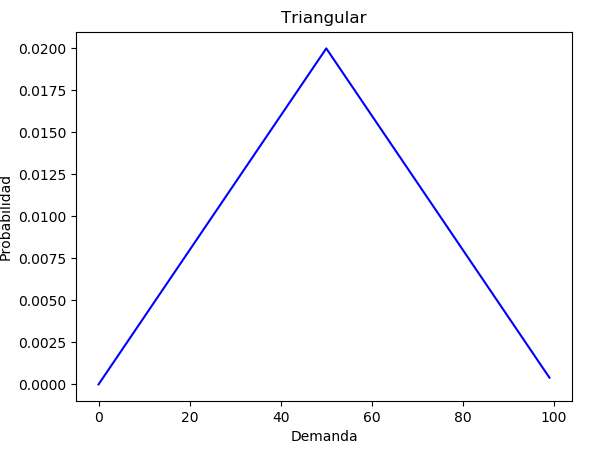
\includegraphics[width=1\linewidth]{img/screenshot002}
	\caption{}
	\label{fig:screenshot002}
\end{figure}
\newpage
La proporcional nos da los peores resultados debido a que se tiene más probabilidad a una demanda más baja que a una demanda alta. Esto se da porque tiene una probabilidad decreciente desde los valores iniciales hasta los valores finales. En la grafica se ve claramente como las demandas más altas tienen muy poca probabilidad de ser obtenida. Esto hace que siempre se vendan menos periódicos y tener unos ingresos menores, por tanto se obtendrá un valor para la demanda optimo más cercana a valores menores que los otros dos modelos.
\begin{figure}[H]
	\centering
	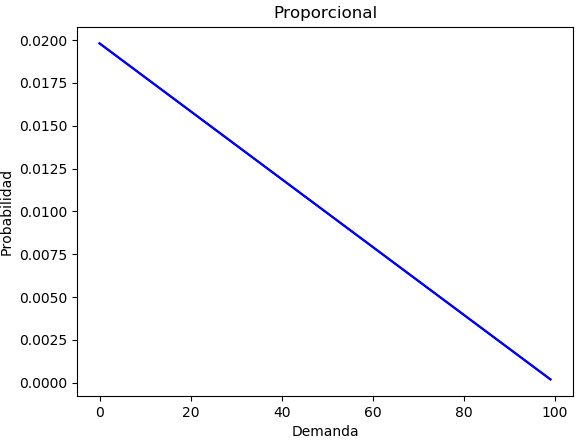
\includegraphics[width=1\linewidth]{img/screenshot001}
	\caption{}
	\label{fig:screenshot001}
\end{figure}
En estos casos como no tenemos la función que nos dice cual seria el optimo como en el caso de la uniforme, otro valor que nos puede indicar que nuestro modelos funcionan bien es que con un valor para las pérdidas (y) mayor se tiende a coger un óptimo menor para no tener tantas pérdidas, y esto también repercute en que las ganancias bajan.
\newline

En el caso de uniforme tenemos la misma probabilidad para todas las opciones, por tanto pueden darse días que se vendan mucho y otros que se vendan menos. Esto hace más difícil asegurarnos que cogemos un valor para s bueno en todos los casos, puesto que si se coge valores pequeños si tenemos una demanda alta en un día no podremos cubrila y en el caso de tener una demanda más baja y tenemos un valor de s muy grande tendríamos muchas más pérdidas. Esto hará que las  ganancias cuando tenemos unas pérdidas por unidad no vendidas pequeñas se acerque más a los valores de la triangular puesto que podemos arriesgarnos a pedir más unidades. En cambio cuando las pérdidas por unidad no vendida son más alta, nos acercaremos más a las ganancias de la proporcional al tener un coste en las pérdidas mayor.

\subsection{Primera Modificación}

El fichero que contiene esta primera modificación es ModeloMontecarloM1. En esta modificación se cambia el parámetro y (perdida por unidad no vendida) por un gasto fijo por devolución(z). Este gasto fijo sera el precio a pagar para devolver cualquier numero de periódicos no vendidos. Siempre que tengamos periódicos sobrantes se pagara este gasto. La función seria la siguiente:



$$
g(s, x, y, d)=\left\{\begin{array}{ll}{x * s} & { { si\ } d \geq s} \\ {x * d-z} & { { si \ } d<s}\end{array}\right.
$$

Solo es necesario cambiar la siguiente parte del condigo:
\begin{figure}[H]
	\centering
	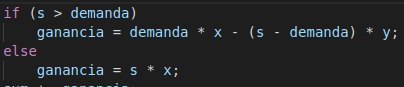
\includegraphics[width=1\linewidth]{img/screenshot003}
\end{figure}

Se añade en la parte del if donde miramos si hay periódicos sobrantes la resta del precio de devolución. Quedando de la siguiente manera:

\begin{figure}[H]
	\centering
	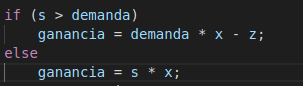
\includegraphics[width=1\linewidth]{img/screenshot005}
	\label{fig:screenshot005}
\end{figure}
\newpage
Vamos a analizar como cambian los ejemplos anteriores con este nuevo cambio. Se repetirá un total de $10^{7}$ veces.

\begin{enumerate}
	\item \textbf{ x = 10 z = 1}
	\begin{table}[H]
		\begin{center}
			
			\begin{tabular}{|l|l|l|}
				
				\hline
				Distribución & Óptimo programa(s) & Mejor ganancia media\\
				\hline \hline
				Uniforme & 99 & 494.061
				\\ \hline
				Proporcional & 98 & 329.057
				\\ \hline
				Triangular & 97 & 499.064
				\\ \hline
				
			\end{tabular}
			
			\label{tabla:sencilla}
		\end{center}
	\end{table}
	\item \textbf{ x = 10  z = 5}
	\begin{table}[H]
		\begin{center}
			\begin{tabular}{|l|l|l|}
				
				\hline
				Distribución & Óptimo programa(s) & Mejor ganancia media\\
				\hline \hline
				Uniforme & 98 & 490.056
				\\ \hline
				Proporcional & 94 & 325.045
				\\ \hline
				Triangular & 96 & 495.122
				\\ \hline
				
			\end{tabular}
			
			\label{tabla:sencilla}
		\end{center}
	\end{table}
	\item \textbf{ x = 10  z = 10}
	\begin{table}[H]
		\begin{center}
			\begin{tabular}{|l|l|l|}
				
				\hline
				Distribución & Óptimo programa(s) & Mejor ganancia media\\
				\hline \hline
				Uniforme & 99 & 485.169
				\\ \hline
				Proporcional & 99 & 320.085
				\\ \hline
				Triangular & 98 & 490.067
				\\ \hline
				
			\end{tabular}
			
			\label{tabla:sencilla}
		\end{center}
	\end{table}
	
\end{enumerate}

En los tres casos se ve como se dan óptimos muy altos, esto se debe a que el precio de devolución es independiente al numero de periódicos no vendidos. Y ademas en estos ejemplos el precio de devolución se costea con las ganancias de la venta de un único periódico. Para ver como cambiara el parámetro z el comportamiento de nuestro simulador, este tendría que ser superior a las ganancias por la venta de varios periódicos. En este caso vamos a realizar una nueva prueba con los siguientes parámetros, x = 10 y z = 150. Con estos valores necesitarías vender al menos 15 periódicos para costear los gastos de devolución.

\begin{table}[H]
	\begin{center}
		\begin{tabular}{|l|l|l|}
			
			\hline
			Distribución & Óptimo programa(s) & Mejor ganancia media\\
			\hline \hline
			Uniforme &  85 & 356.991
			\\ \hline
			Proporcional & 69 & 184.928 
			\\ \hline
			Triangular & 70 & 360.058
			\\ \hline
			
		\end{tabular}
		
		\label{tabla:sencilla}
	\end{center}
\end{table}

Con esto vemos como al subir el coste de la devolución, el simulador vuelve a quedarse con valores más pequeños de s. Esto se da porque intenta limitar las unidades a pedir para no tener que realizar devoluciones, ya que tienen un coste muy elevado. Esto significa que se pierdan posibles ventas al quedarnos sin periódicos para ahorranos la devolución.

\subsection{Segunda Modificación}
Para esta modificación se ha utilizado el fichero ModeloMontecarloM2.Para la modificación tendremos en cuenta que hay veces en los que el número de periódicos que no hemos vendido nos reporta una perdida menor al precio fijado para la devolución. Para esto se utiliza la siguiente función:
$$
g(s, x, y, d)=\left\{\begin{array}{ll}{x * s} & { { si \ } d \geq s} \\ {x * d-\min \{z,(s-d) * y\}} & { { si \ } d<s}\end{array}\right.
$$

Necesitamos modificar el mismo if del apartado anterior añadiendo la nuevas opciones, quedando de esta manera:

\begin{figure}[H]
	\centering
	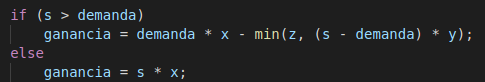
\includegraphics[width=1\linewidth]{img/screenshot006}
	\label{fig:screenshot006}
\end{figure}


Vamos a realizar un ejemplo para ver el funcionamiento del nuevo modelo. 
Para esto utilizaremos los siguintes valores {x = 10 z = 150 y = 1 }. Escojo esta x y z para que coincidan con el ultimo ejemplo del apartado anterior. Pongo una y baja para que pueda decidir quedarse los periódicos no vendidos antes de devolver estos y pagar más.  
	\begin{table}[H]
		\begin{center}
			\begin{tabular}{|l|l|l|}
				
				\hline
				Distribución & Óptimo programa(s) & Mejor ganancia media\\
				\hline \hline
				Uniforme &  91 &  449.72
				\\ \hline
				Proporcional & 79  & 464.236
				\\ \hline
				Triangular & 78  & 464.239
				\\ \hline
				
			\end{tabular}
			
			\label{tabla:sencilla}
		\end{center}
	\end{table}
	
Como se ve en comparación del ejemplo anterior. Todos las distribuciones de probabilidad han dado mejores resultados que el apartado donde nos forzaba a devolver los periódicos sobrantes con el coste que esto conlleva. Esto se debe a que en determinados casos con una z alta, como este caso, es preferible quedarse los periódicos sobrantes a pagar por devolverlos.
\newpage
\subsection{Mejoras de Tiempo}
En este apartado veremos como realizando tres pequeñas optimizaciones reducimos el tiempo de ejecución y lo importante que es esto cuando necesitamos simular muchas acción.

\subsubsection{Ordenar en Orden Decreciente.}
La mejora viene enfocada en la creación de las tablas de probabilidad. Generaremos las tablas de forma decreciente en probabilidad. Estando primero los valores que tengan mayor probabilidad de tocar. 
Un pequeño ejemplo seria el siguiente:

$$P(a) = 0.3, P(b) = 0.5, P(c) = 0.2$$
\newline
Con estos datos nuestro tabla tendría que tener primero el valor b, después a y por ultimo c. Como en nuestro caso estamos usando una búsqueda lineal recorriendo la tabla de principio a fin, si al principio tenemos los valores con más probabilidad, parara la búsqueda en más ocasiones antes de llegar a la parte final de la tabla. Por ejemplo si nuestro primer tercio del vector tiene valores que entre todos ellos tienen una probabilidad del 70\% de ser elegidos, el 70\% de las veces no miraremos los dos últimos tercios de la tabla de probabilidad.
\newline

Para esto necesitaremos modificar la tabla para que almacene tanto el rango de números que le pertenece según su probabilidad y el numero al que pertenece. Esto lo he solucionado creando un struct que almacene estos dos valores y creando la tabla de probabilidades de el tipo struct que he creado. 
\newline

Esta mejora solo se puede dar para el caso de la probabilidad triangular puesto que las otras dos casos ya están ordenadas de este modo por su propia definición.

Con esto ya tendríamos solucionado todo lo pedido para esta mejora. Vamos a pasar a ver la mejora en tiempo.

\begin{table}[H]
	\begin{center}
		\begin{tabular}{|l|l|l|}
			
			\hline
			Nº de Repeticiones & Sin mejora(s) & Con mejora(s)\\
			\hline \hline
			$10^{2}$ & 0.005094  &  0.003771
			\\ \hline
			$10^{3}$ & 0.031151  &  0.030161
			\\ \hline
			$10^{4}$ & 0.16533  &  0.124196
			\\ \hline
			$10^{5}$ & 1.64078 &  1.20811
			\\ \hline
			$10^{6}$ &  16.4164 &  12.2003
			\\ \hline
			$10^{7}$ & 164.025  &  121.142
			\\ \hline
		\end{tabular}
		
		\label{tabla:sencilla}
	\end{center}
\end{table}

Como se ve la mejora es grande en tamaños en repeticiones muy elevadas cosiguiendo mejorar hasta 40 segundos $10^{7}$

\subsubsection{Cambiar el Tipo de Búsqueda}
En este caso aprovechamos que las tablas por defectos viene ordenadas con números entre el rango [0,1] para implementar en vez de la búsqueda lineal dada en el código otra búsqueda más eficiente. Para esto utilizamos la búsqueda binaria que cambiamos de O(n) de la búsqueda lineal a O($log(n)$). Vamos a comparar la mejora en tiempo de ejecución.

\begin{table}[H]
	\begin{center}
		\begin{tabular}{|l|l|l|}
			
			\hline
			Nº de Repeticiones & Sin mejora(s) & Con mejora(s)\\
			\hline \hline
			$10^{2}$ & 0.005094  &  0.002774
			\\ \hline
			$10^{3}$ & 0.031151  &  0.025144
			\\ \hline
			$10^{4}$ & 0.16533  &  0.089586
			\\ \hline
			$10^{5}$ & 1.64078 &  0.835823
			\\ \hline
			$10^{6}$ &  16.4164 &  8.68748
			\\ \hline
			$10^{7}$ & 164.025  &  85.9786
			\\ \hline
		\end{tabular}
		
		\label{tabla:sencilla}
	\end{center}
\end{table}

En este caso tenemos una reducción en el tiempo de ejecución de casi el doble. Esto se debe al cambio de O(n) a O(log(n))

\subsubsection{Probabilidad Uniforme en O(1)}
En este caso para la probabilidad uniforme tenemos la tabla de probabilidad de tamaño n. Y dentro de este tabla tenemos n números en el rango[0,1] con una separación de 1/n. Esto no es necesario puesto que podemos obtener el número que corresponde a estar probabilidad se puede hacer con operaciones matemáticas pasando de O(n) a O(1). Las operación seria una división de u, un número aleatorio generado de forma uniforme entre [0,1], y n que es el total de números posibles. Después devolvemos la parte entera de esta división.Vamos a comparar la mejora en tiempo de ejecución.

\begin{table}[H]
	\begin{center}
		\begin{tabular}{|l|l|l|}
			
			\hline
			Nº de Repeticiones & Sin mejora(s) & Con mejora(s)\\
			\hline \hline
			$10^{2}$ & 0.005075  &  0.001256
			\\ \hline
			$10^{3}$ & 0.031608  &  0.010205
			\\ \hline
			$10^{4}$ & 0.161896  &  0.046164
			\\ \hline
			$10^{5}$ & 1.64078 &  0.328868
			\\ \hline
			$10^{6}$ &  16.2737 &  3.20168
			\\ \hline
			$10^{7}$ & 158.824  &  31.9284
			\\ \hline
		\end{tabular}
		
		\label{tabla:sencilla}
	\end{center}
\end{table}

Esta es la mejora más eficiente bajando casi 150 segundos el tiempo de ejecucion al pasar de O(n) a O(1). El problema de esta mejora es que solo se puede dar cuando tenemos una distribución de probabilidad que podamos obtener a cual pertenece con cálculos matemáticos sencillos sin el uso de bucles. Esto no se puede realizar en todos los casos.

\section{Generadores Congruenciales}

Vamos a realizar pruebas con los dos siguientes generadores congruenciales:

$$
x_{n+1}=\left(2060 x_{n}+4321\right) \mathrm{mod} m
$$
 
$$
x_{n+1}=\left(2061 x_{n}+4321\right) \mathrm{mod} m
$$
	
Lo primero que necesitaremos es iniciar los valores para $x^{0}$, en este caso yo he iniciado con el valor 14. Otro valor que necesitamos elegir sera el valor de m. En la práctica nos especifica que utilicemos el valor 10000. 

Una vez iniciados estos parámetros podemos pasar a ver los ciclos de estos generadores. En la siguiente tabla mostrare los ciclos de los generadores.

\begin{table}[H]
	\begin{center}
		\begin{tabular}{|l|l|l|}
			
			\hline
			Generador & Generador con 2061 & Generador con 2060\\
			\hline \hline
			Entero & 10000  &  5
			\\ \hline
			Real Artesanal Float & 298 &  9
			\\ \hline
			Real Artesanal Double & 235  &  5
			\\ \hline
			Real Artesanal Corregido & 10000 &  5
			\\ \hline
			Real con Fmod & 10000  & 5
			\\ \hline
		\end{tabular}
		
		\label{tabla:sencilla}
	\end{center}
\end{table}

Los valores que han llegado a 10000 quiere decir que han conseguido generar todos los números sin repetirlos. Los que han parado antes de 10000 son por encontrar un numero repetido. En este caso el generador con el valor 2060 no es un buen generador puesto que ninguno de ellos ha llegado a 10000. Esto se da porque para que un generador congruencias no repita números hasta que genere todos los valores del modulo el valor m que es 10000 y 2060 tendrían que ser primos realitos y no lo son. En el caso de 2061 y 10000 son primos relativos y por eso si llega a completar ciclos sin repetir un numero. 

En la tabla anterior se ve como ademas los generadores artesanales con double y float no llegan a completar un ciclo entero sin repetir parando antes que los demás para el primer generador. Esto se debe a la precisión de los tipos de datos usados. Para evitar podríamos redondear como en el Artesanal corregido o hacer la comparación restando los dos números y viendo que dan un valor menor a un numero especificado como posible error. Ademas en este caso float y double no fallan en el mismo numero porque tienen una precisión distinta.


\end{document}


